\documentclass[12pt, varwidth, border=5mm]{standalone}
\usepackage{tikz}
\usepackage{amsmath}
% Underlining package
\usepackage{ulem}
\usetikzlibrary{calc}
\usetikzlibrary{angles,quotes}
% \usepackage[a4paper, portrait, margin=1cm]{geometry}

\begin{document}
\section*{ }
    \begin{minipage}{0.55\textwidth}
  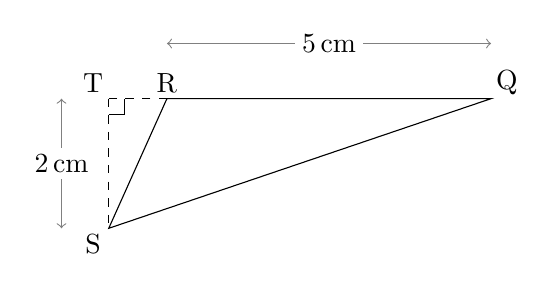
\begin{tikzpicture}[scale=1.0, baseline=(current bounding box.north)]
    \begin{scope}[rotate=180]

        \coordinate (Q) at (0,0);
        \coordinate (R) at (4.117,0);
        \coordinate (T) at ($(R)+(0.739,0)$);  % extend out
        \coordinate (S) at ($(T)+(0,1.647)$); % Perpendicular upwards

        \draw (Q)--(R)--(S)--cycle;
        \draw[dashed] (R)--(T);
        \draw[dashed] (T)--(S);
        \pic [draw, -, angle radius=0.2cm] {right angle=S--T--R};

        % Vertex LABELS
        % Labels relative to shape geometry
        \node at ($(Q)+(-0.2,-0.2)$) {Q};
        \node at ($(R)+(0.0,-0.2)$) {R};
        \node at ($(T)+(0.2,-0.2)$) {T};
        \node at ($(S)+(0.2,0.2)$) {S};


        % dotted/dashed arrows shifted away from edges
        % Horizontal side (A-B), shifted down yshift=0mm,
        \draw[<->, gray]
            ($(Q) + (0,-0.7cm)$) -- ($(R) + (0,-0.7cm)$)
            node[black, midway, fill=white, inner sep=2.5pt] {5\,cm};

        % Vertical side (D-C), shifted right xshift=0mm,
        \draw[<->, gray]
            ($(T)+(0.6,0)$) -- ($(T |- S)+(0.6,0)$)
            node[black, midway, fill=white, inner sep=2.5pt] {2\,cm};

    \end{scope}
\end{tikzpicture}
\end{minipage}%
\hfill
\begin{minipage}{.4\textwidth}
  \begin{align*}
    \text{Area} &= \frac{1}{2} \text{bh} \\
    \text{Area} &= \frac{1}{2} \times 5 \text{cm} \times 2 \text{cm}  \\
    \text{Area} &= 5.0 \text{cm}^2
  \end{align*}
\end{minipage}

\end{document}
